\chapter{Schramm-Loewner Evolutions}
\label{ch4-sle}

Lorem ipsum dolor sit amet, consectetur adipisicing elit, sed do eiusmod tempor
incididunt ut labore et dolore magna aliqua. Ut enim ad minim veniam, quis
nostrud exercitation ullamco laboris nisi ut aliquip ex ea commodo consequat.
Duis aute irure dolor in reprehenderit in voluptate velit esse cillum dolore eu
fugiat nulla pariatur. Excepteur sint occaecat cupidatat non proident, sunt in
culpa qui officia deserunt mollit anim id est laborum.

\section{Loewner Evolutions}
\label{sec:le}

Loewner were proposed by Charles Loewner in the context of Bierbach
conjecture (today called de Branges's theorem) in the 1920's.

In Section [???] we described how the perimeter of percolation cluster can be
generated using an exploration process. Loewner evolutions represent the
continuum limit of such processes.

\begin{equation}
    \partial_t g_t(z) = \frac{2}{g_t(z) - U_t}
    \label{eq:loew}
\end{equation}


\begin{figure}
\begin{center}
    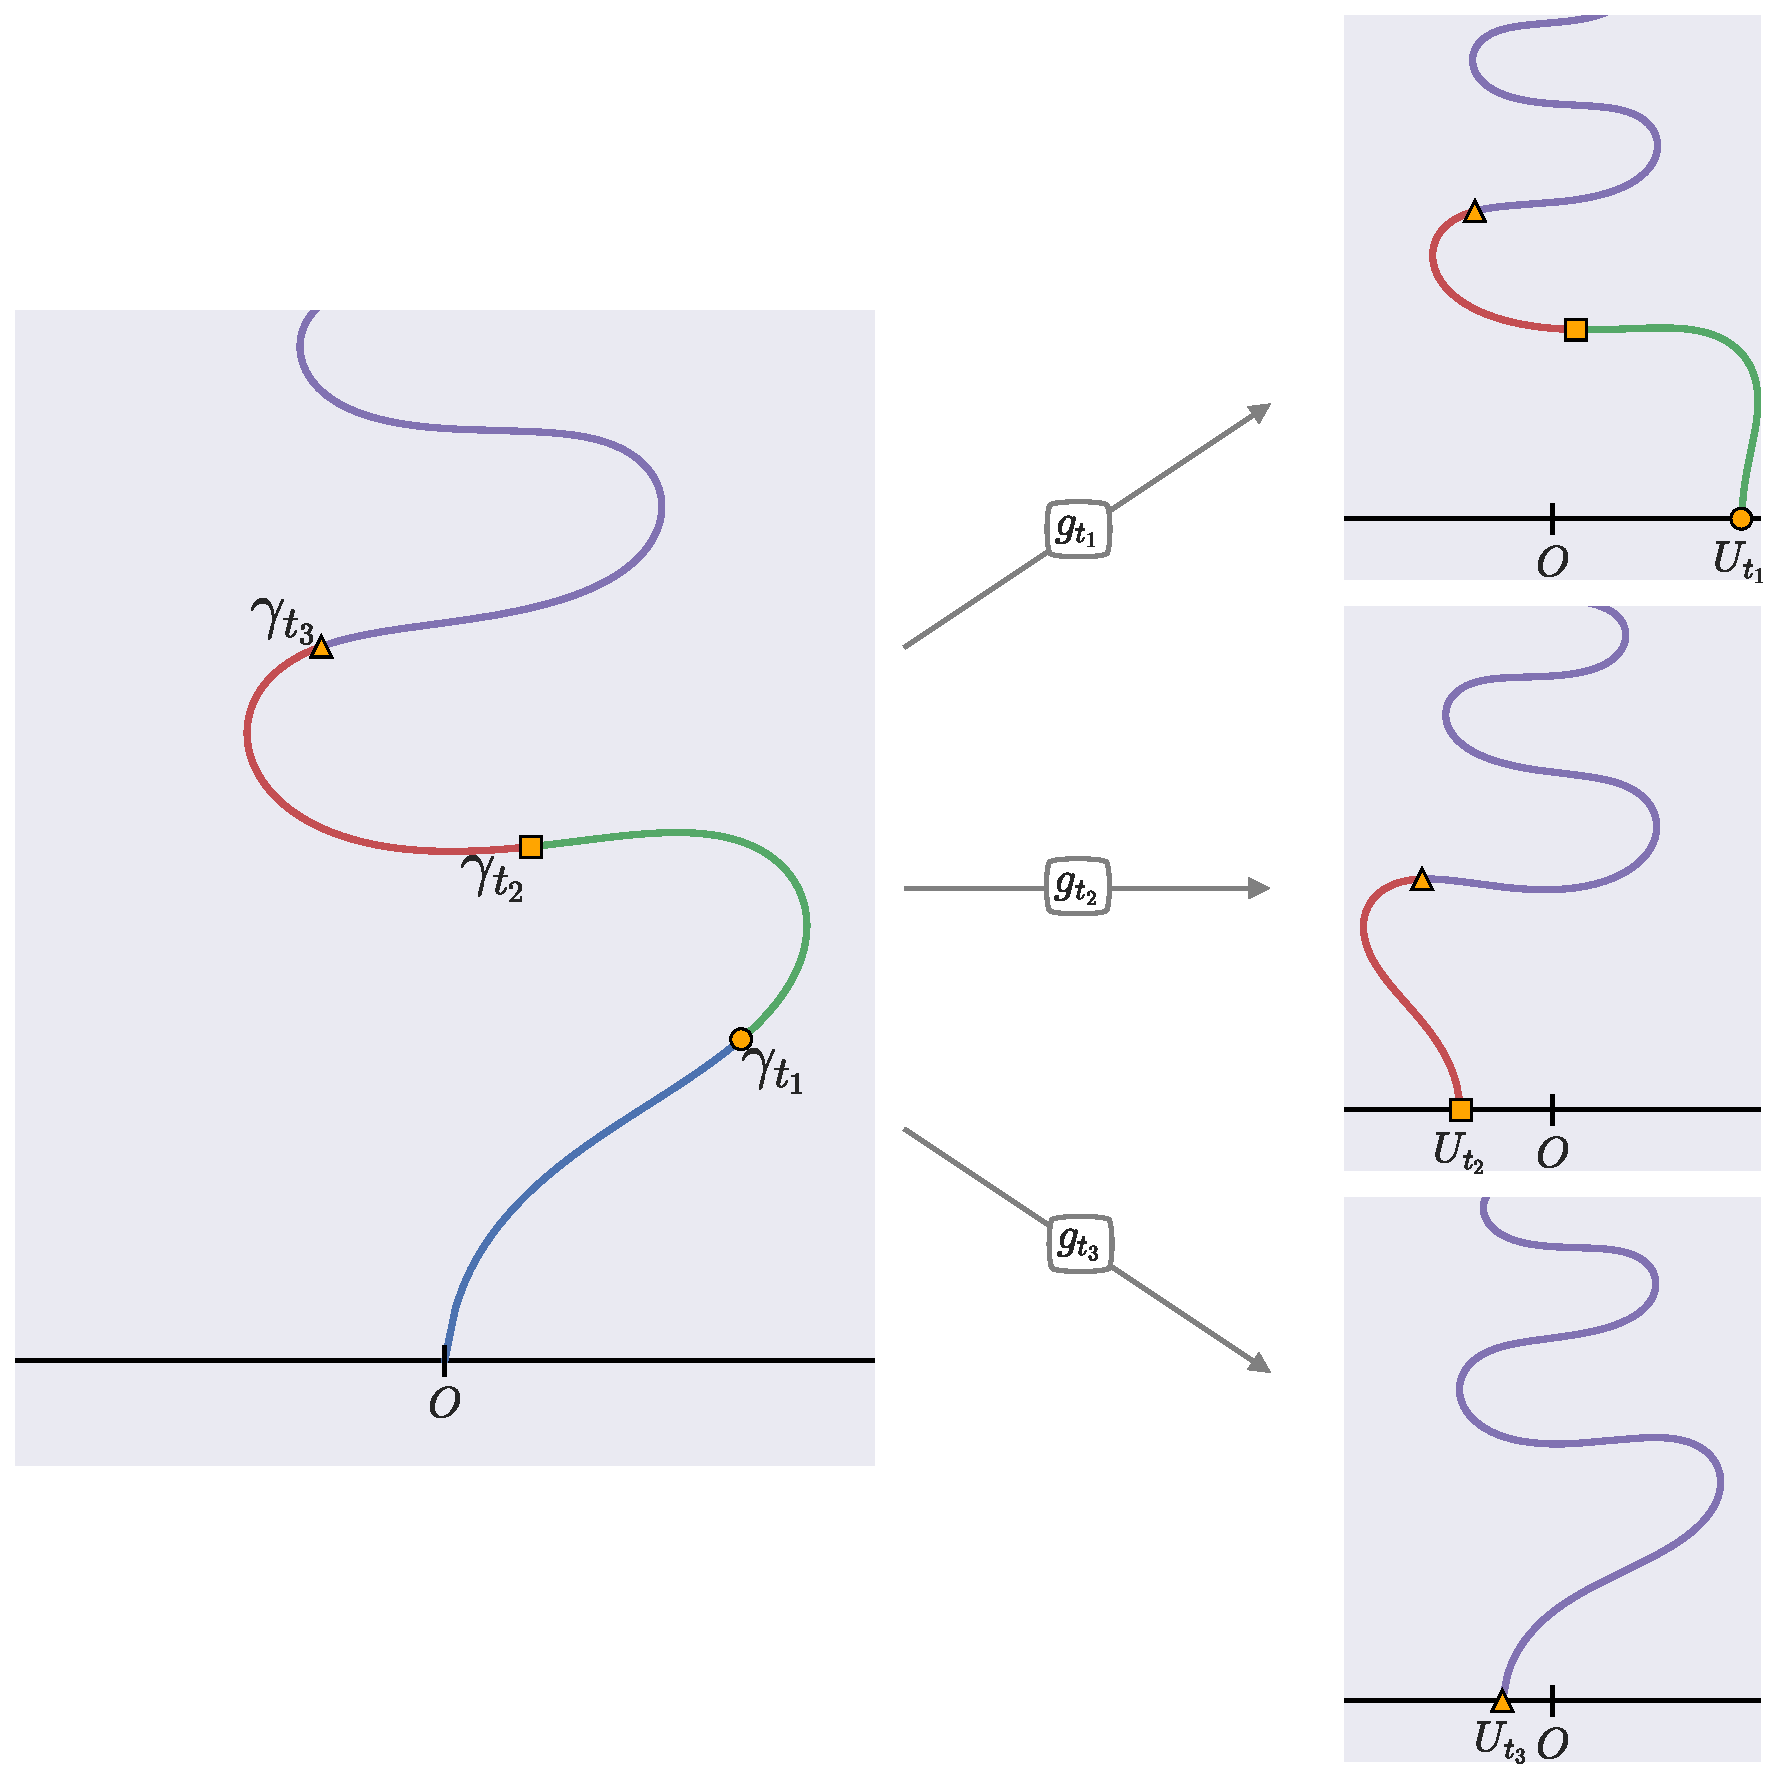
\includegraphics[scale=0.4]{chapters/ch4-sle/figs/loewexplain}
\end{center}
\caption{How the chordal Loewner evolution works. We define the trace $\gamma$
    parametrized by a time $t$. At each time instant there is a conformal map
    $g_t$ that maps the upper half plane minus the trace up to time $t$ to the
    upper half plane itself, that is, $g_t:\HH\setminus\gamma_{[0,t]}
    \rightarrow\HH$. The tip of the trace always get mapped to the real line.
    If we track the point where the tip is mapped, we get a function $U_t$
    called driving function, in mathematical terms
    $U_t=g_t\left(\gamma_t\right)$.}
\label{fig:loewexplain}
\end{figure}


\section{Stochastic Loewner Evolutions}
\label{sec:le}

\textbf{Coformal Invariance.}
We talked extensively in Chapter~\ref{ch3-conf} about conformal invariance and
its importance to the study of critical systems. There we used a field
theoretical approach, but in the context of measure theory, conformal
invariance is stated as
\begin{equation}
    \newcommand{\pp}[1]{\left(#1\right)}
    f\circ\mu_D\pp{z,w} = \mu_{f(D)}\pp{f\pp{z}, f\pp{w}}.
\end{equation}
This is to say, given a domain $D$ and a set of curves $\gamma$ that connect
the points $z$ and $w\in\partial D$, the measure $\mu$ of this family of curves
is invariant under a conformal transformation $f$. In simpler words, it means
that if you have a certain (continuum) model $M$ and use it to generate a set
of curves in $D$ and then conformally map the curves to $f(D)$, these
curves would have the same statistical properties as if you simply generated the
curves by applying $M$ to $f(D)$ directly. An illustration can be seen in
Figure~\ref{fig:confinv}.


\textbf{Domain Markov Property.}
In his work, Schramm identified another fundamental property that conformally
invariant lattice models tend to obbey called domain Markov property. It
stated as
\begin{equation}
    \newcommand{\pp}[1]{\left(#1\right)}
    \mu_D\pp{\gamma_2|\gamma_1} = \mu_{D\setminus\gamma_1}\pp{\gamma_2}.
\end{equation}
That is, the conditional measure of family of curves $\gamma_2$ that have the
same start $\gamma_1$ in a domain $D$ is the same as that of $\gamma_2$ in
a domain with $\gamma_1$ removed, that is, $D\setminus\gamma_1$.
In the same line of conformal invariance, domain Markov property can be
understood in the following way: if you have a model M and use it to generate a
set of curves in $D$ that all have the same start $\gamma_0$, the curves
$\gamma_1$ obtained would have the exact same properties as if you generated
the curves by applying M to $D\setminus\gamma_0$. An illustration can be
seen in Figure~\ref{fig:dmp}.

\begin{figure}
\begin{center}
    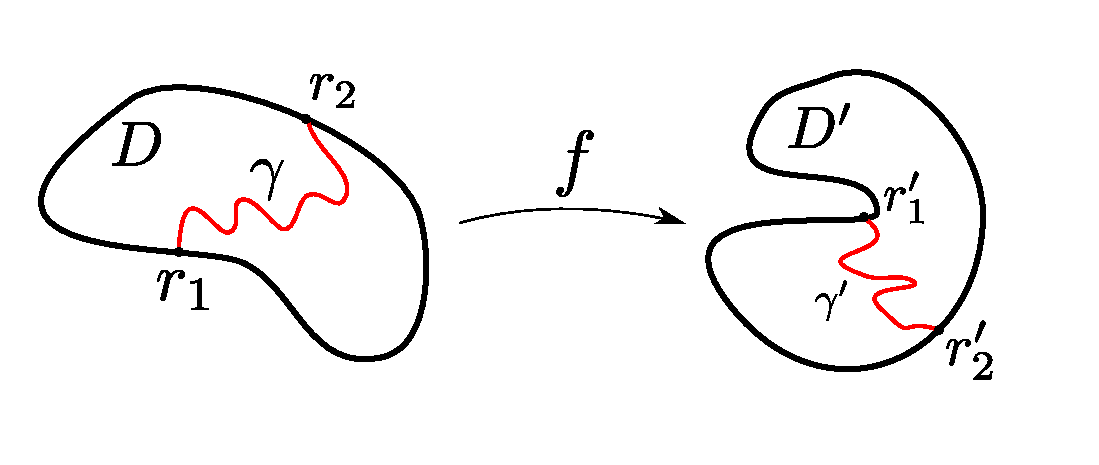
\includegraphics[scale=0.8]{chapters/ch4-sle/figs/confinv}
\end{center}
\caption{Lorem ipsum dolor sit amet, consectetur adipisicing elit, sed do
    eiusmod tempor incididunt ut labore et dolore magna aliqua. Ut enim ad
    minim veniam, quis nostrud exercitation ullamco laboris nisi ut aliquip ex
    ea commodo consequat. Duis aute irure dolor in reprehenderit in voluptate
    velit esse cillum dolore eu fugiat nulla pariatur. Excepteur sint occaecat
    cupidatat non proident, sunt in culpa qui officia deserunt mollit anim id
    est laborum.}
\label{fig:confinv}
\end{figure}


\begin{figure}
\begin{center}
    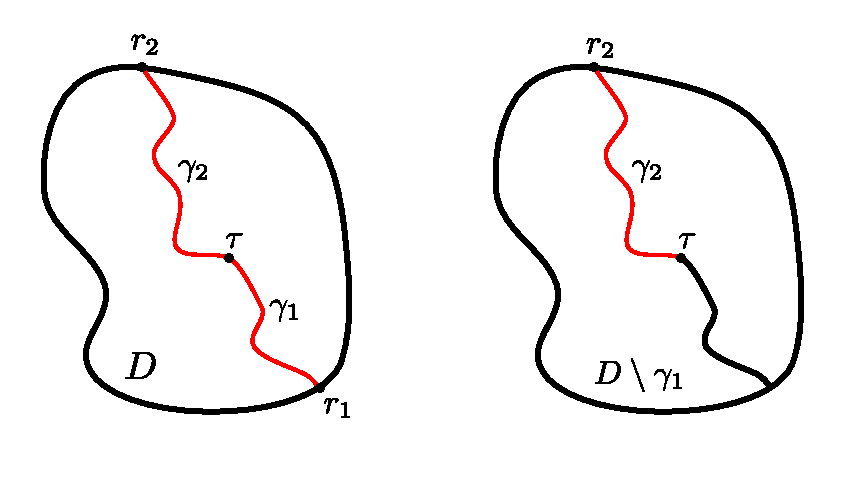
\includegraphics[scale=0.9]{chapters/ch4-sle/figs/dmp}
\end{center}
\caption{The domain Markov property states that the conditional measure of
    $\gamma_2$ given a fixed $\gamma_1$ in a domain $D$ is the same of $\gamma_2$
    in the same domain with $\gamma_1$ removed, that is, $D\setminus\gamma_1$.}
\label{fig:dmp}
\end{figure}


\section{Numerical Methods}
\label{sec:num}

The crux of the Schramm Loewner Evolution problem is determining whether or not
a given model converges to it in the continuum limit, and what is the value of
$\kappa$ for this specific model. We mentioned several models that have been
proven to asdasd, the most illustrious being Smirnov's demonstration that
percolation in a triangular lattice converges to SLE with $\kappa=6$.

Nonetheless, just like nobody would expect every critical system to have an
exact solution similar to the Ising model, one may not expect to be able to
prove the SLE convergence for every conceivable model. To be completely
fair, we cannot there is no way to know this prove is impossible either, but

This is where
numerical analysis comes into the scene. By comparing the statistical behavior
of the model with the expected SLE trace, we can infer Eq.~\ref{eq:prob} holds
true.

\subsection{Euler's Method}
\label{ss:euler}

Euler's method for solving ordinary differential equations is arguably the
simplest. It is used to solve equation of the type $y'(t) = f(y, t)$ and it
basically consists in taking a first order approximation of the solution
\begin{equation}
    \newcommand{\y}[1]{y\left(#1\right)}
    \newcommand{\f}[1]{f\left(#1\right)}
    \y{t} = \y{t_0} + \int_{t_0}^t \f{\y{\tau}, \tau} d\tau \approx
            \y{t_0} + \left(t - t_0\right)\f{\y{t_0}, t_0}.
\end{equation}
This way, the equation can be solved recursivelly by providing a discretized
driving function $U_{t_i}$ with $t_0 = 0 < t_{1}<\cdots<t_N$ and. Applying it
to Loewner's equation (Eq.~\ref{eq:loew}) we have
\begin{equation}
    g_{t_{i+1}}(z) = g_{t_i}(z) + (t_{i+1} - t_i) \frac{2}{g_t(z) - U_{t_i}}.
\end{equation}

In order to obtain the trace from $g_t$ we take the fact that
\begin{equation}
    g_t(\gamma_t) = U_t.
    \label{eq:root}
\end{equation}
You can use your favorite method of root finding to solve Eq.~\ref{eq:root} for
$\gamma_t$. In Figure~\ref{fig:euler1} you can see a realization for
$\kappa=2$. In it we colored the grid according to the sign of
$Re\{g_t(z)-U_t\}$. The border between the positive and negative sides should
be around the region where the trace is. We also observe the most blatant
drawback of the method: it fails in several points, where they get mapped
outside the upper half plane, which is not allowed in chordal Loewner's
evolutions. This problem accentuates quickly as the value of $\kappa$ rises,
to the point where the case $\kappa=6$ (Figure~\ref{fig:euler2}) has barely
any discernible trace.

Other problem with Euler's method in the context of Loewner evolutions is
computational complexity. It requires $O(N)$ for each point of the space where
you compute $g_t(z)$, considering the you use a $(M,M)$ regular grid, the whole
algorithm have complexity $O(NM^2)$. This is further aggravated by the fact the
most points are not necessary to actually compute the trace, making most of the
computational effort useless. One possible advantage is the fact that this
algorithm is highly parallelizable, although this is hardly an advantage faced
with the other drawbacks.

\begin{figure}
\begin{center}
    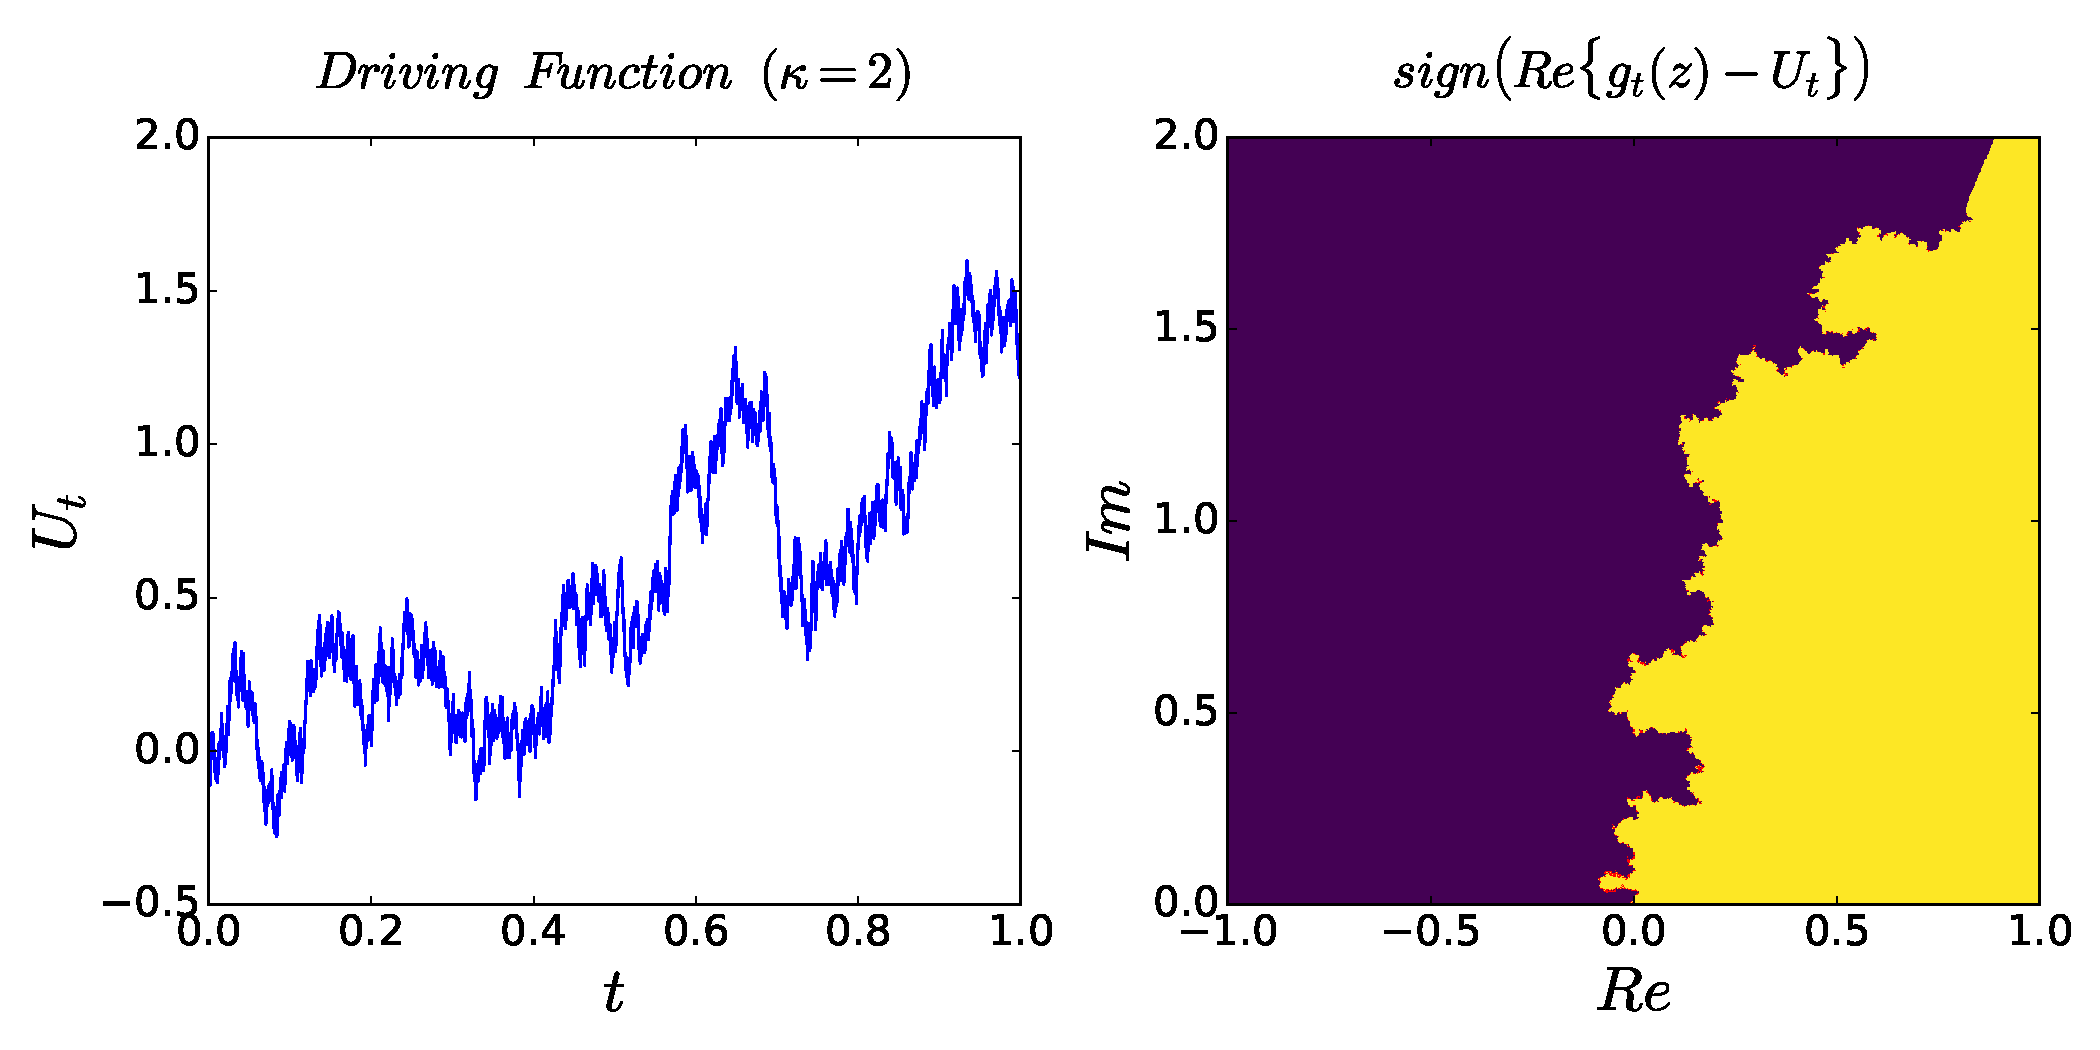
\includegraphics[scale=0.45]{chapters/ch4-sle/figs/euler1}
\end{center}
\caption{Simulation of an SLE process with $\kappa=2$ using the Euler method
    with $\Delta t = 10^{-5}$ in a grid of resolution $(1024, 1024)$. Because
    at time $t$ $g_t(\gamma_t)-U_t=0$, if we color the upper half plane
    according to which side of the real line each point is mapped, the border
    between the regions should indicate the position of the trace $\gamma_t$.
    The red points are the points where the method failed and were mapped
    outside the upper half plane. The smooth ``tail'' of the trace happens
    because these points have not yet been mapped to the real line.}
\label{fig:euler1}
\end{figure}

\begin{figure}
\begin{center}
    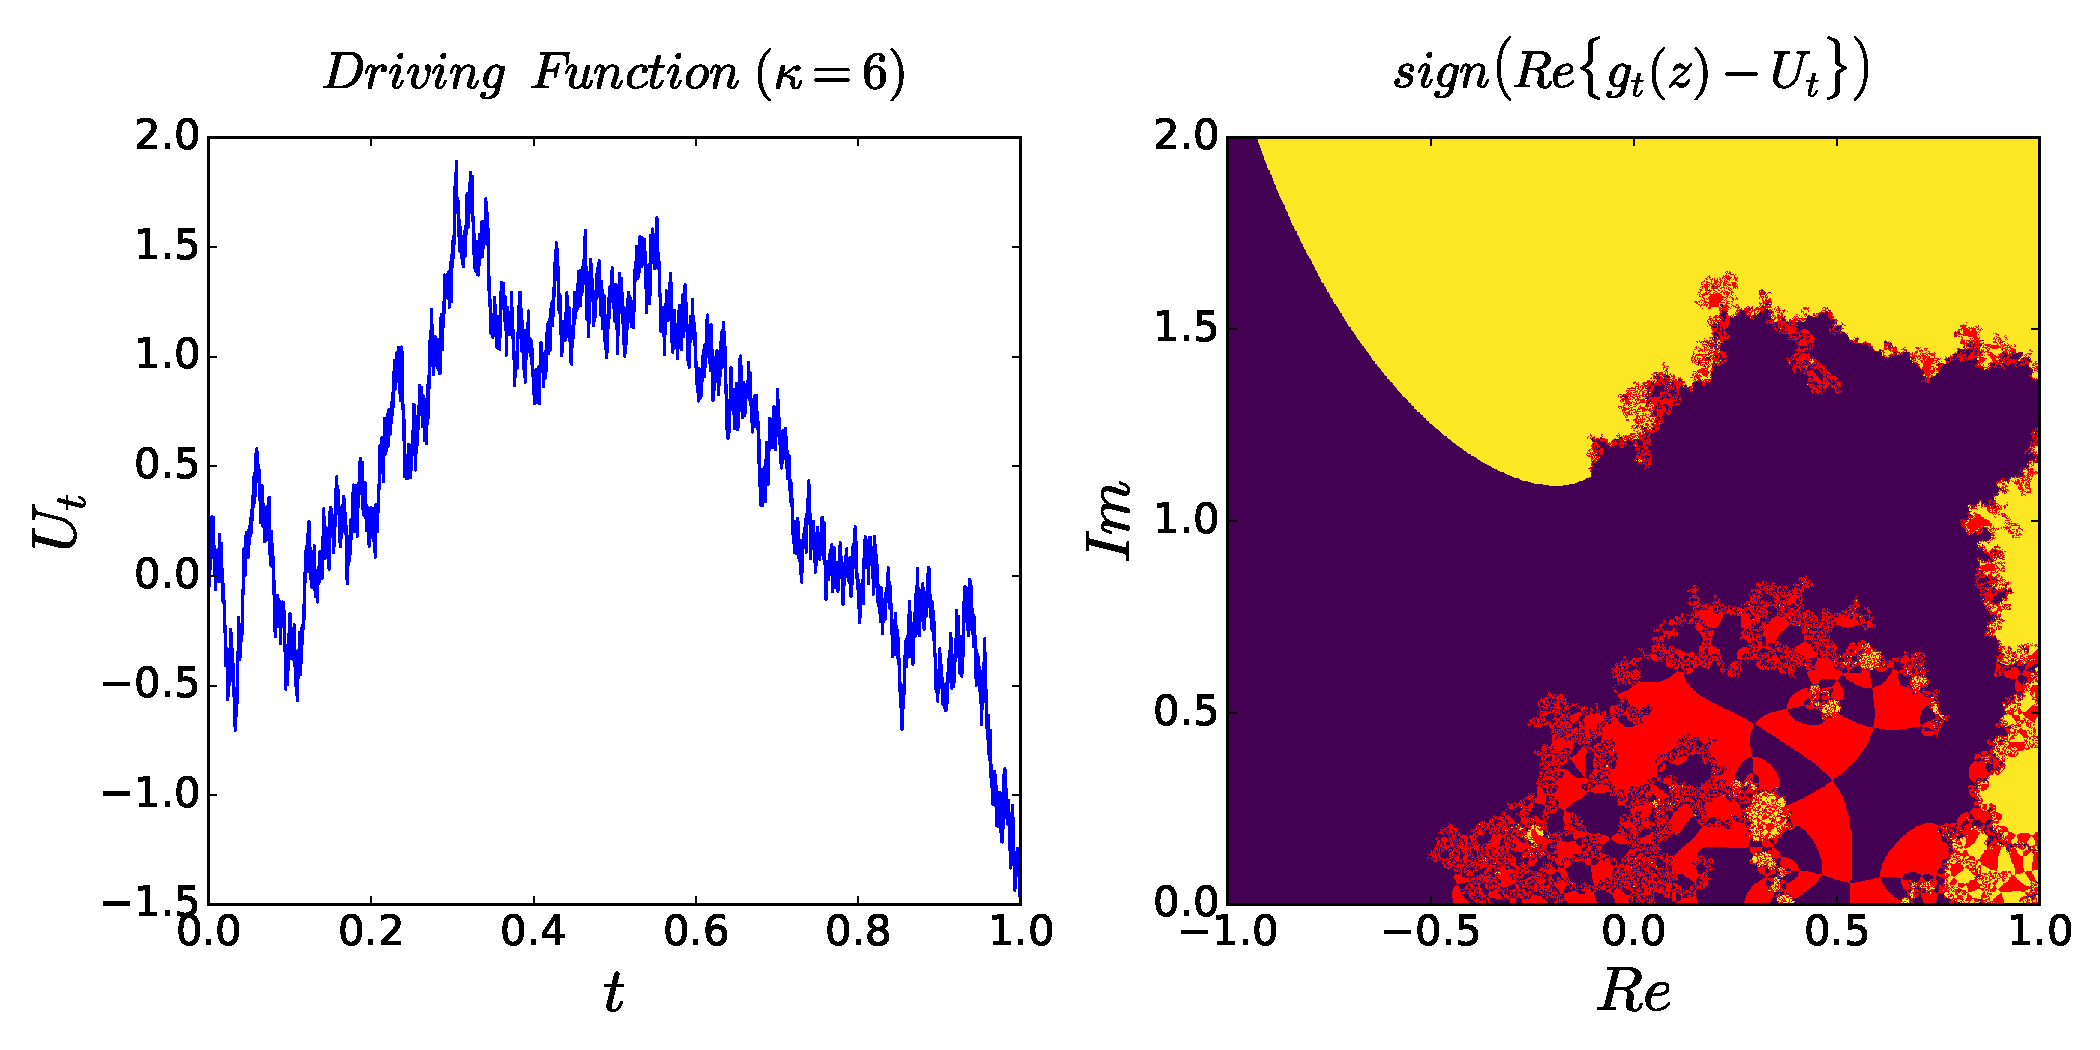
\includegraphics[scale=0.45]{chapters/ch4-sle/figs/euler2}
\end{center}
\caption{Simulation of an SLE process with $\kappa=6$ using the Euler method
    with $\Delta t = 10^{-5}$ in a grid of resolution $(1024, 1024)$. 
    The red points are the points where the method failed and were mapped
    outside the upper half plane. The algorithm performed much worse than
    the case $\kappa=2$.}
\label{fig:euler2}
\end{figure}


\subsection{Zipper Algorithm}
\label{ss:zipper}

Since the Euler's method perform so poorly in the task of computing the SLE
trace, a better method is needed. The one described here is called the
\textit{zipper algorithm}, and it's used throughout this work. It is based on
the idea of discreet Loewner evolutions [???], basically consisting in breaking
the Loewner evolution of the full trace in a series of smaller simpler Loewner
evolutions.

For starters, we take a driving function $U_t$ sampled in a set of $N+1$ time
instants $0=t_0<t_1<\cdots<t_N$. As we already established, the solution of the
Loewner's equation for $U_t$ is $g_t$, which maps
$\HH\setminus\gamma_{\left[0,t_{k}\right]}$ to $\HH$. We then define the
helper function
\begin{equation}
    G_{k}=g_{t_{k}}\circ g_{t_{k-1}}^{-1},
\end{equation}
which maps $\HH\setminus\gamma_{\left[0,t_{k-1}\right]}$ to
$\HH\setminus\gamma_{\left[0,t_{k}\right]}$. This way the solution of Loewner's
equation can be rewritten
\begin{equation}
    g_{t_{k}}=G_{k}\circ G_{k-1}\circ\cdots\circ G_{2}\circ G_{1}.
\end{equation}
The $G_k$ however are not solutions of Loewner's equation, as the trace they
generate do not start at the origin. We fix that by shifting the function by
$U_{t_{k-1}}$
\begin{equation}
    g_{k}=G_{k}\left(z+U_{t_{k-1}}\right)-U_{t_{k-1}}.
\end{equation}
Note that in the notation adopted (taken from [???]) $g_{t_k}$ and $g_k$ are
different functions. The $g_k$ are the solution of Loewner's equation with
driving function $\tilde{U}_t$ such that $\tilde{U}_0=0$ and $\tilde{U}_{\Delta
t_k} = \Delta U_k$, where $\Delta t_k = t_{k} - t_{k-1}$ and $\Delta U_{k}
= U_{k} - U_{k-1}$. Since we are trying to construct the trace starting from
the drive, we need to take the inverse of $g_k$
\begin{equation}
    f_{k}=G_{k}^{-1}\left(z+U_{t_{k-1}}\right)-U_{t_{k-1}}.
\end{equation}
The $k$-th point of the trace $\gamma_{t_k}$ is then determined by 
\begin{equation}
    \gamma_{t_k} = f_1(\cdots f_{k-1}(f_k(\Delta U_k)+\Delta U_{k-1})\cdots+\Delta U_1).
\end{equation}
For convenience we define
\begin{equation}
    h_{k}=f_{k}\left(z+\Delta U_{k}\right),
\end{equation}
so the $\gamma_t$ can be computed by applying the relation
\begin{equation}
    \label{eq:zip}
    \gamma_{k}=h_{1}\circ h_{2}\circ\cdots\circ h_{k}\left(0\right).
\end{equation}
If this helper function zoo looks confusing, Figure~\ref{fig:zipperdiag} shows
where they fit in the actual Loewner evolution process taking place.

Once the functional form of the $h_k$ is know, the algorithm is surprisingly
simple, it just consists of applying Eq.~\ref{eq:zip} for each value of $k$.
The form of $h_k$ however is dependent on the interpolation drive $\tilde{U}$.
The choice is basically free, however a convenient one should have an
analytical solution. The two most common are the vertical and tilted slits.

The vertical slit is done by making
\begin{equation}
    \tilde{U}(t)=\Delta U,
\end{equation}
which generate a vertical trace going from $\Delta U$ to $\Delta U +
i2\sqrt{\Delta t}$. This isn't strictly a Loewner evolution because the trace
does not start at the origin, but this is a numerical approximation where the
actual trace is a composition of many vertical slits, and the limit $\Delta t
\rightarrow 0$ converges to an actual SLE trace. The $h_k$ in this case is
given by
\begin{equation}
    \label{eq:vslit}
    h_{k}(z)=i\sqrt{4\Delta t-z^{2}}+\Delta U.
\end{equation}

The tilted slit is done by interpolating the drive with the function.
\begin{equation}
    \tilde{U}(t)=
        \frac{2\left(1-2\alpha\right)}
             {\sqrt{\alpha\left(1-\alpha\right)}}
        \sqrt{t}
\end{equation}
where
\begin{equation}
    \alpha=\frac{1}{2}-
    \mbox{sign}\left(\Delta U\right)\frac{1}{2}\sqrt{\frac{v}{16+v}},
    \,\,\,\,\,\,\,\,\,\,\,\,\,\,
    v=\frac{\Delta U^{2}}{\Delta t}.
\end{equation}
It generates a trace that is a tilted line that starts at the origin makes an
angle $\alpha\pi$ with the positive real line. The $h_k$ in this case is
given by
\begin{equation}
    h_{k}(z) = 
    {\left(
        z+2\sqrt{\frac{\left(1-\alpha\right)\Delta t}{\alpha}}
    \right)}^{1-\alpha}
    {\left(
        z-2\sqrt{\frac{\alpha\Delta t}{1-\alpha}}
    \right)}^{\alpha}.
\end{equation}
This discretization is more rigorous than the vertical slit, however in
practice they yield very similar results. See Figure~\ref{fig:zipper} for an
illustration of the whole process of applying repeated tilted slits to obtain
an SLE trace.

You can see in Figure~\ref{fig:eulerzip} how the zipper algorithm performs in
the high $\kappa$ regime. The result is not perfect, the jump size
$\left|\gamma_{k}-\gamma_{k-1}\right|$ is very non-uniform due to the high
volatility of the driving function. Nevertheless, the result is still much
better than the one obtained by using Euler's method, and the defects can be
mitigated by simply adding more points to the discretized driving function.
This is not so simple, however. Since each $k$-th point require $k$ application
of the $h_i$, the algorithm scales as $O(N^2)$, which can get unwieldy
for very large $N$. One possible solution is making use of parallelization,
since each $\gamma_k$ can be computed independently from one another.

The next challenge is to do the opposite task, obtaining a driving function
from a given trace $\gamma_k$. This is much simpler when using a vertical slit.
First let's invert Equation~\ref{eq:zip}
\begin{equation}
    \label{eq:unzip1}
    0=h_{k}^{-1}\circ h_{k-1}^{-1}\circ\cdots h_{1}^{-1}\left(\gamma_{k}\right).
\end{equation}
We know that the vertical slit maps the origin to $\Delta U+i2\sqrt{\Delta t}$,
that is
\begin{equation}
    \label{eq:unzip2}
    h_{k}\left(0\right)=\Delta U+i2\sqrt{\Delta t}.
\end{equation}
Combining Eq.~\ref{eq:unzip1} and Eq.~\ref{eq:unzip2} we have    
\begin{equation}
    \Delta U_{k}+i2\sqrt{\Delta t_{k}}=
    h_{k-1}^{-1}\circ\cdots h_{1}^{-1}\left(\gamma_{k}\right).
\end{equation}
This way we can determine the $t_k$ and $U_{t_k}$ of given discretized
trace by simply taking
\begin{equation}
    t_{k}=\sum_{i=1}^{k}\mbox{Re}\left\{ \omega_{i}\right\},
    \,\,\,\,\,\,\,\,\,\,
    U_{t_{k}}=\frac{1}{4}\sum_{i=1}^{k}\mbox{Im}\left\{ \omega_{i}\right\} ^{2}
\end{equation}
where
\begin{equation}
    \omega_{k}=h_{k-1}^{-1}\circ h_{k-2}^{-1}\circ
        \ldots\circ h_{1}^{-1}\left(\gamma_{k}\right).
\end{equation}
The $h_k^{-1}$ can be easily determined by inverting Eq.~\ref{eq:vslit}
\begin{equation}
    h_{k}^{-1}\left(z\right)=
    i\sqrt{-Im{\left\{ \omega_{k}\right\}}^{2}
           -{\left(z-\mbox{Re}\left\{ \omega_{k}\right\} \right)}^{2}}.
\end{equation}


\begin{figure}
\begin{center}
    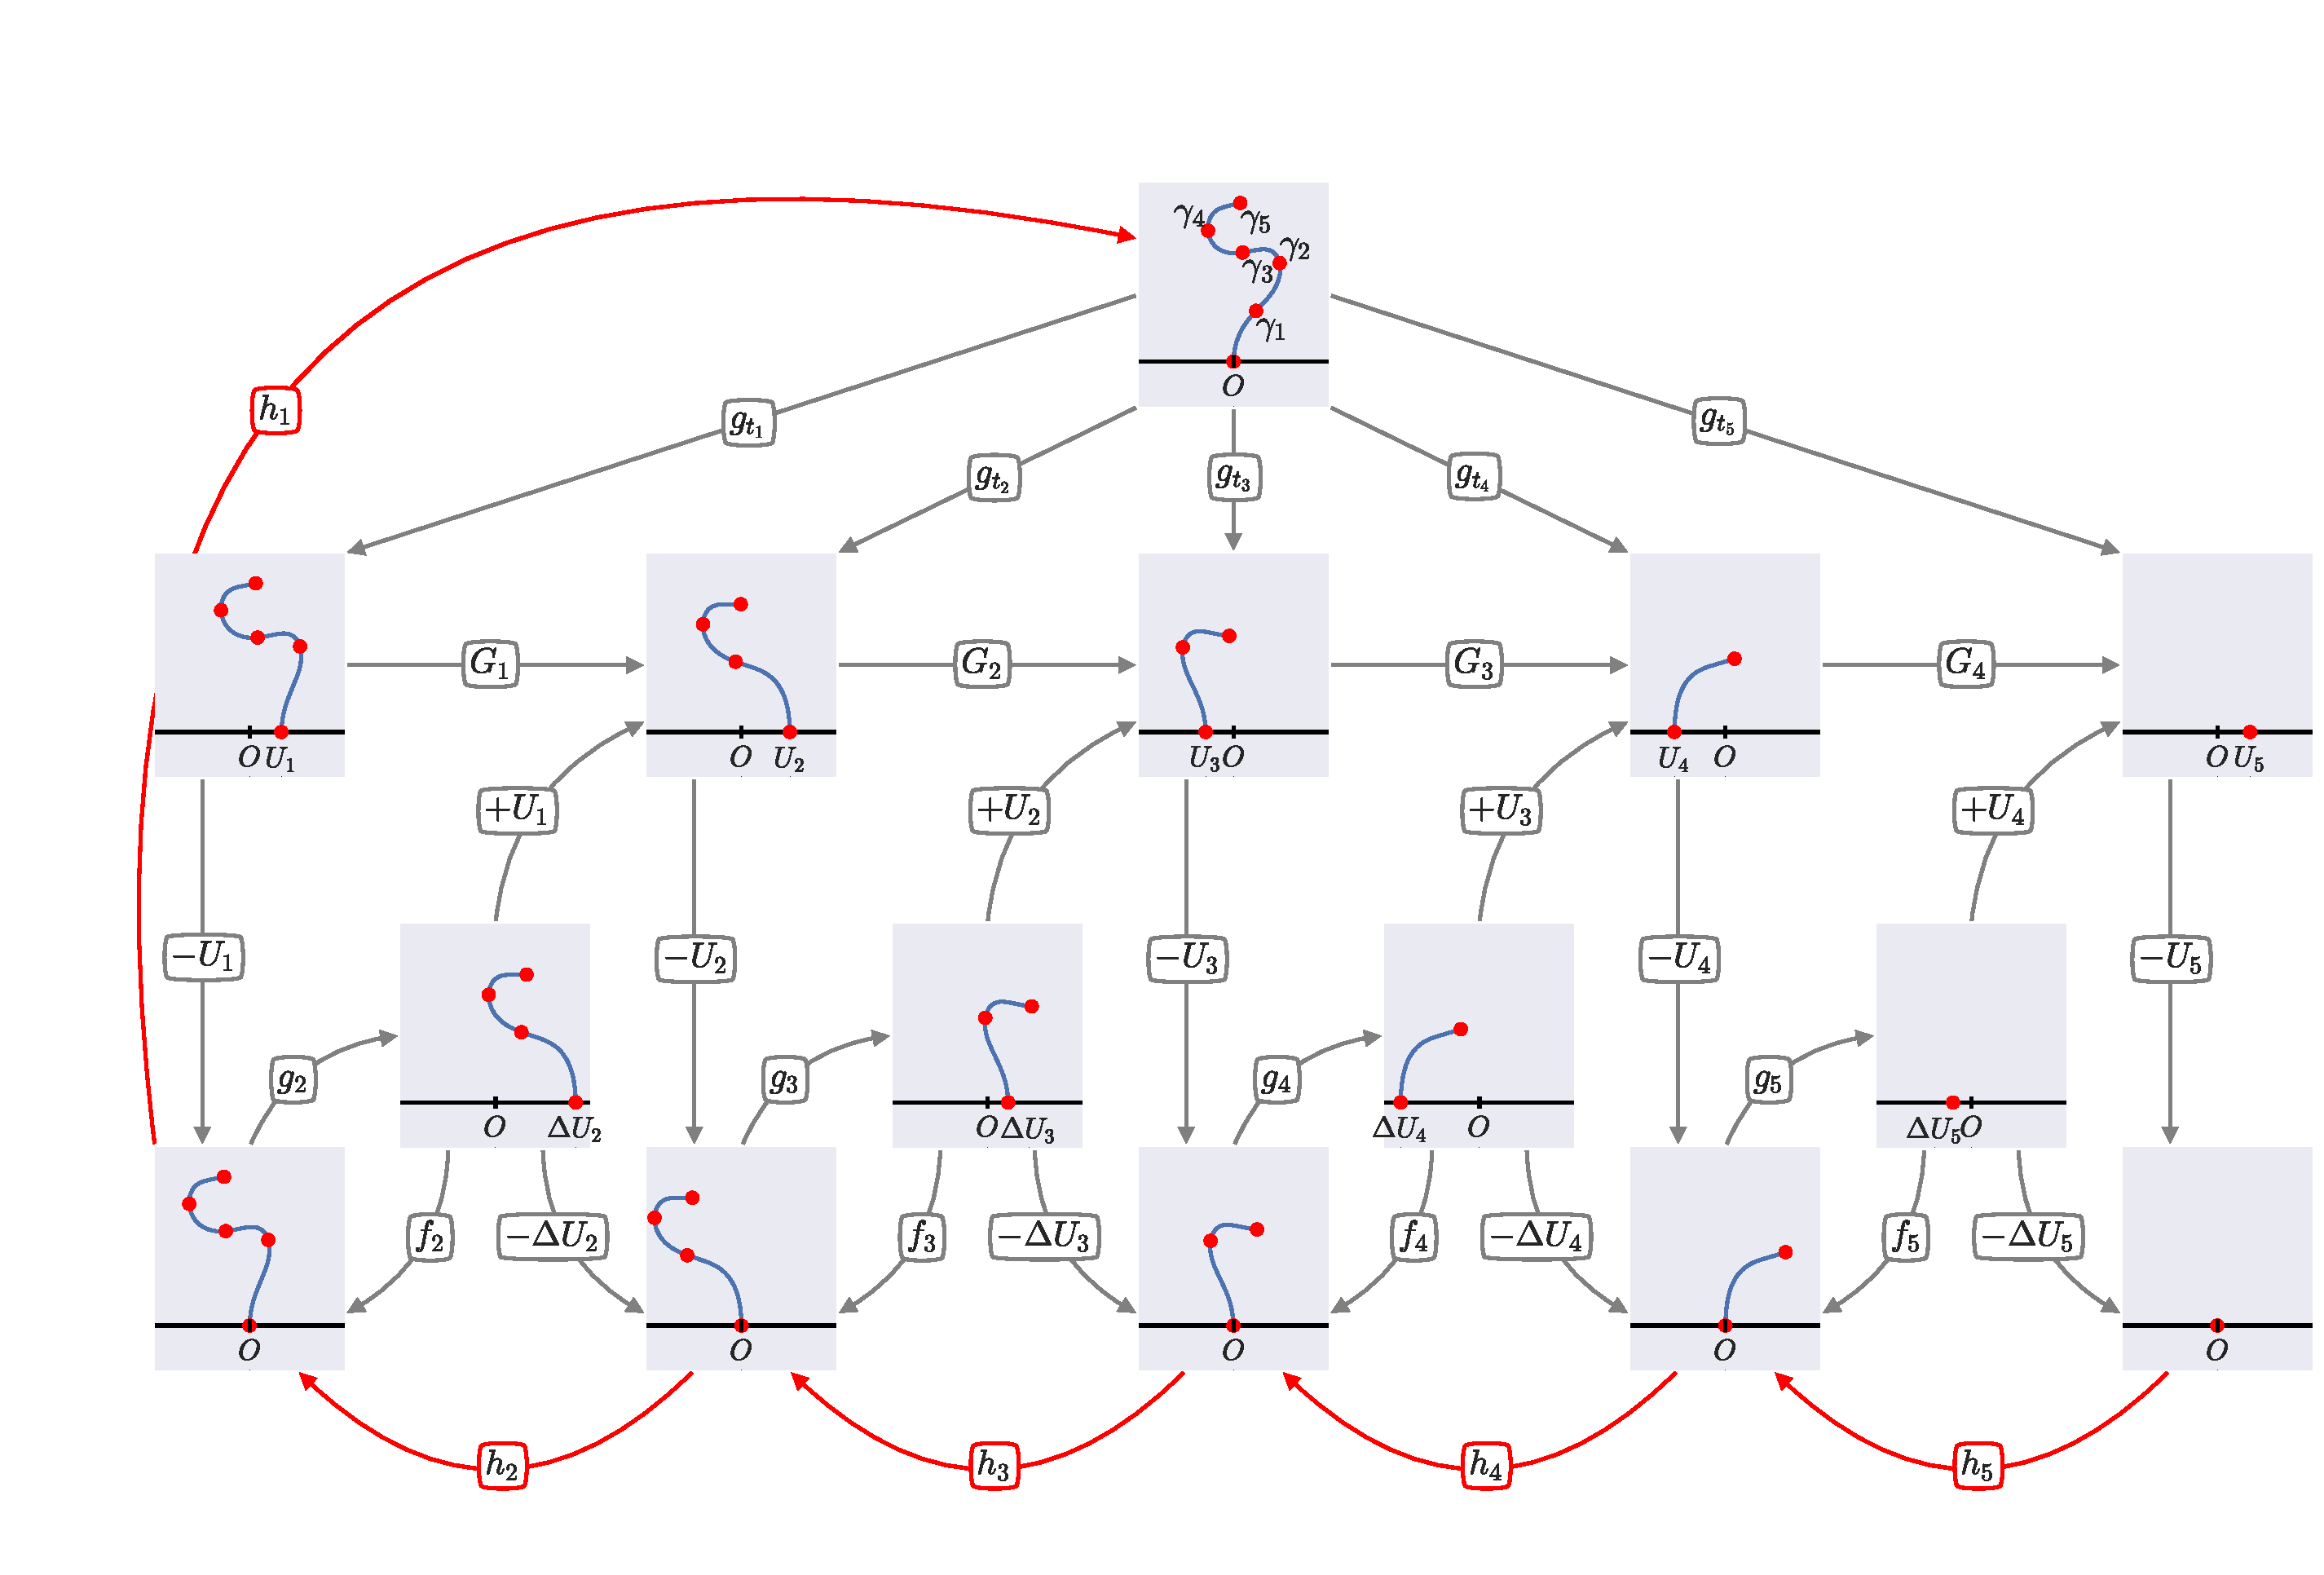
\includegraphics[scale=0.34]{chapters/ch4-sle/figs/zipperdiag}
\end{center}
\caption{Schematic representation of how the zipper algorithm fits in the
    Loewner evolution framework. At the top, we have the full trace up to time
    $t_5$, which we want to reach starting from the empty upper half plane
    (right most panel on the fourth row). To compute the trace from a given
    discretized driving function, one must take the red path. This is achieved
    by using the interpolating maps $g_i$ that are the solution of the Loewner
    equation with driving function $\tilde{U}_0=0$ and $\tilde{U}_{\Delta
    t}=\Delta U$. The choice of interpolation function $\tilde{U}$ is
    arbitrary, but usually taken from the few options that have an analytical
    solution.}
\label{fig:zipperdiag}
\end{figure}

\begin{figure}
\begin{center}
    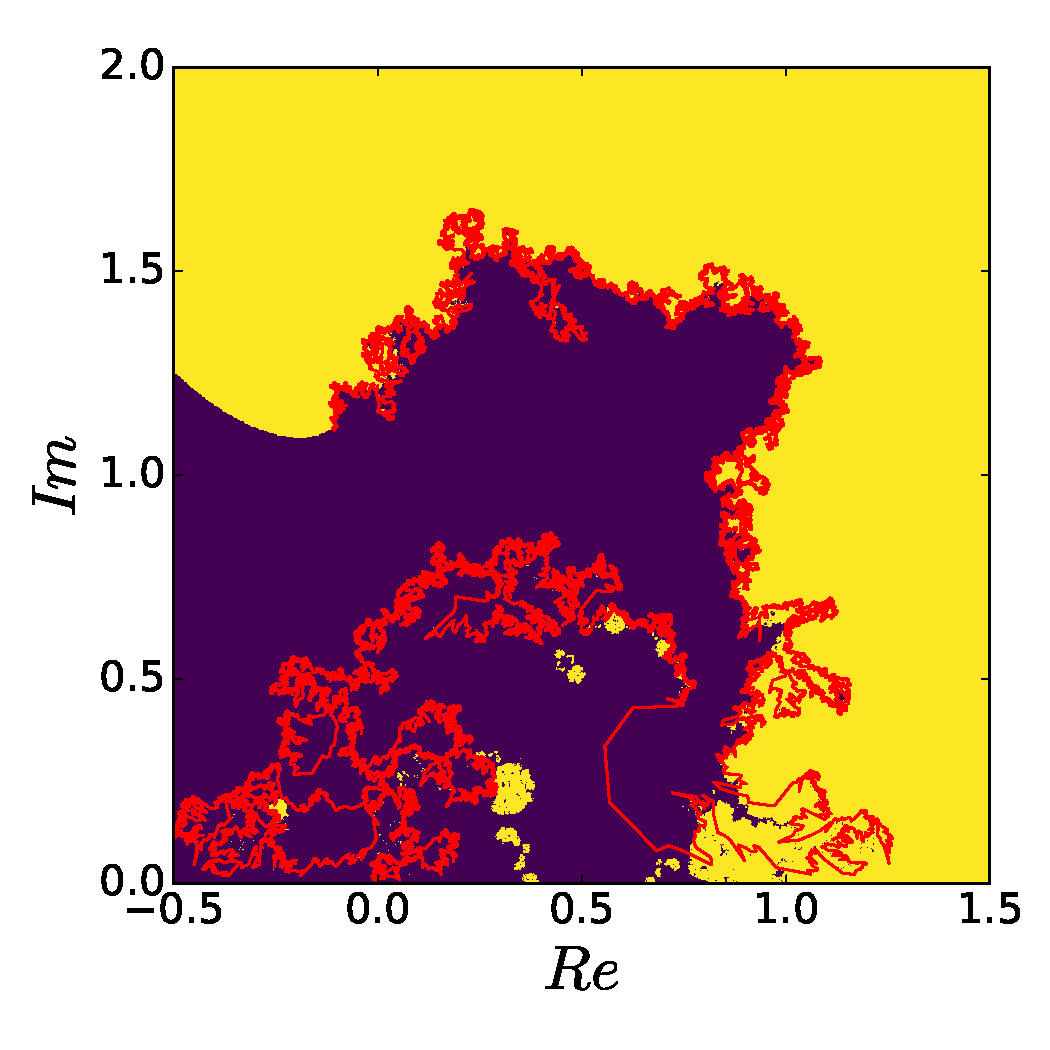
\includegraphics[scale=0.5]{chapters/ch4-sle/figs/eulerzip}
\end{center}
\caption{Comparison of the traces obtained by using the zipper algorithm (red
    line) and Euler's method. Although it presents large jumps in the trace due
    to large displacements in the driving function, zipper it still performs
    better than the Euler's.}
\label{fig:eulerzip}
\end{figure}

\begin{figure}
\begin{center}
    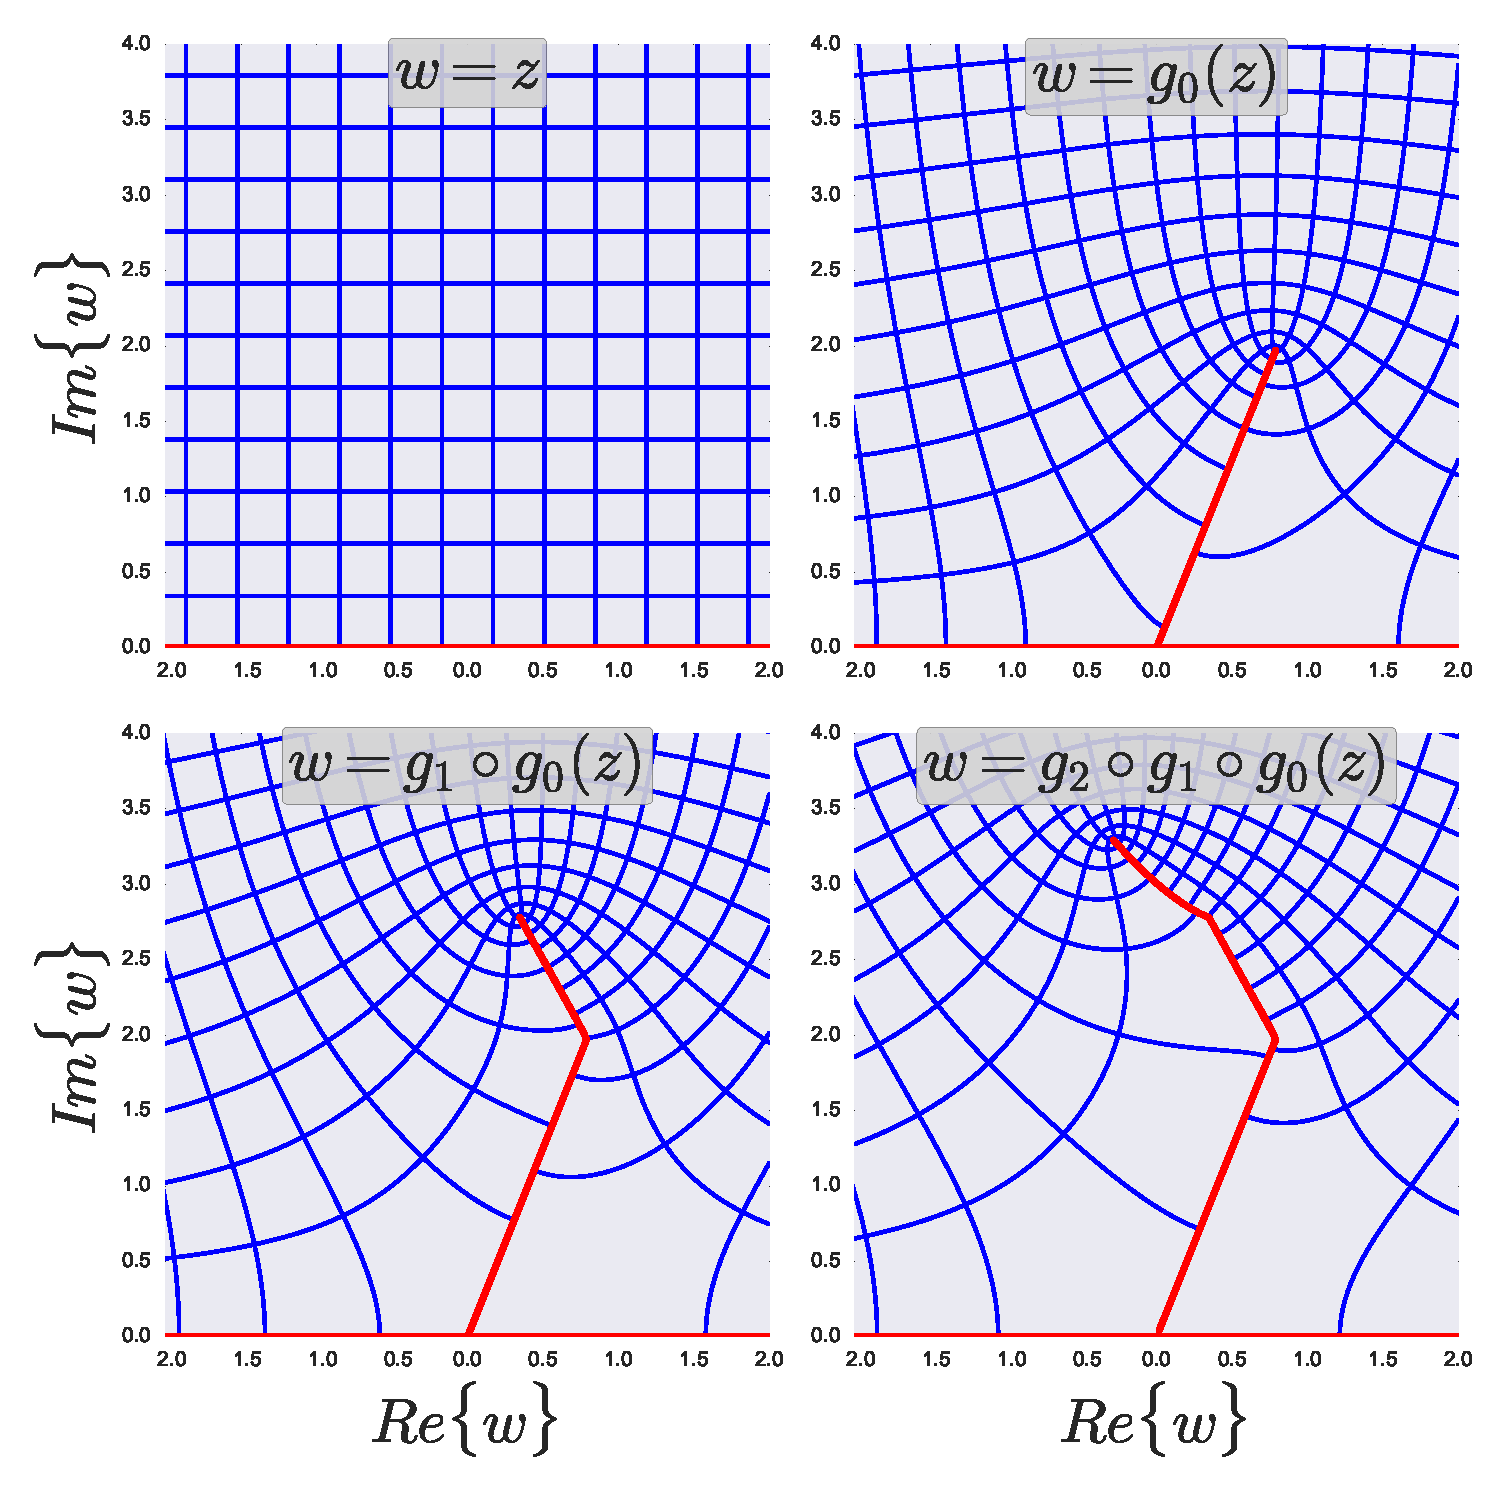
\includegraphics[scale=0.5]{chapters/ch4-sle/figs/zipper}
\end{center}
\caption{Result of applying the first three iterations of the zipper algorithm
    with the tilted slit approximation. In the limit $\Delta t\rightarrow 0$
    the red line converges to an SLE trace.}
\label{fig:zipper}
\end{figure}
